\documentclass[12pt,a4paper]{article}
\usepackage[hyperref]{acl2021}
\usepackage{times}
\usepackage{latexsym}
\renewcommand{\UrlFont}{\ttfamily\small}

\usepackage{microtype}
\usepackage{xcolor}
\usepackage{algorithm} 
\usepackage{amsmath}
\usepackage{algpseudocode}
\usepackage{graphicx}

\aclfinalcopy % Uncomment this line for the final submission
%\def\aclpaperid{***} %  Enter the acl Paper ID here

%\setlength\titlebox{5cm}
% You can expand the titlebox if you need extra space
% to show all the authors. Please do not make the titlebox
% smaller than 5cm (the original size); we will check this
% in the camera-ready version and ask you to change it back.

\newcommand\BibTeX{B\textsc{ib}\TeX}

\let\SUP\textsuperscript
\title{Multi-Domain Meta Calibration Using Differentiable Expected Calibration Error}
\author{$ \begin{matrix} \text{Niv Kook} \\ 211873468 \end{matrix} $\qquad\qquad\qquad $ \begin{matrix} \text{Rotem Ben Zion} \\ 211324975 \end{matrix} $\\[\bigskipamount]
	\{niv.ko, rotm\}@campus.technion.ac.il}

\date{Oct 2022}

\begin{document}
	
\maketitle
\begin{abstract}
Confidence calibration – the problem of predicting probability estimates representative of the true correctness likelihood – is important for classification models in many applications. An existing paper called "Meta-Calibration: Learning of Model Calibration Using
Differentiable Expected Calibration Error" uses meta-learning techniques to train neural networks to be well-calibrated.
In this project, we extend that work to the setting of multiple domains; We define and implement a label-smoothing meta learning technique for multiple domains, and test its calibration generalization quality in over-parameterized neural networks.
\end{abstract}

\section{Introduction}
\label{sec:Introduction}
	When deploying neural networks to real-world applications, it is crucial that models’ own confidence estimates accurately match their
	probability of making a correct prediction. If a model is over-confident about its predictions, we cannot rely on it; while well-calibrated
	models can abstain or ask for human feedback in the case of uncertain predictions. In addition, some tasks directly rely on calibration such as outlier detection \citep{hendrycks2016baseline}. Unfortunately, over-parameterized neural networks tend to be badly calibrated on new data \citep{guo2017calibration}.
	This challenge of calibrating neural networks has motivated a growing area of research, some of the existing methods will be discussed in section \ref{sec:RelatedWork}. One of the promising techniques alters the loss function by introducing label smoothing \citep{muller2019does}, though it is not clear how to choose the smoothing hyper-parameters.
	This motivated the authors of "Meta-Calibration: Learning of Model Calibration Using Differentiable Expected Calibration Error" \citep{bohdal2021meta} to develop a meta-learning technique which allows training a small amount of meta parameters for label smoothing. The training loss is a differetiable approximation of the ECE metric, which is also developed in \cite{bohdal2021meta}. \\
	The difference between train and test calibrations can be viewd in terms of distribution shift and out-of-domain generalization.
	In this project, we test the meta-learning method of \cite{bohdal2021meta} in a multi-domain setting. We compare it to the baseline (no label smoothing) and to a new version, with seperate meta-parameters for each domain. Our goal is to test whether meta-learning the label-smoothing parameters in different domains improves calibration as measured by Average-ECE.

\section{Related work}
\label{sec:RelatedWork}
\subsection*{Calibration}
\label{ssec:calibration}
Model calibration is a popular area of research in recent years. \cite{guo2017calibration} study a variety of potential solutions and find that simple post-training rescaling of the logits – temperature scaling – works relatively well. Other methods, including the ones we implement in this project, apply during model training. This includes the MMCE kernel-base calibration measure provided in \cite{kumar2018trainable} which they use as regularization, the Focal loss \citep{mukhoti2020calibrating} which is a relatively simple weighted alternative to cross-entropy, and the classic Brier score \citep{brier1950verification}, which is the squared error between the softmax vector with probabilities and the ground-truth one-hot encoding. \\
A more relevant work to our project is \cite{muller2019does}, in which label smoothing has been shown to improve model calibration. However, this calibration metric was not optimized as most aforementioned calibration metrics are non-differentiable. The work of \cite{bohdal2021meta} does optimize the calibration metric as will be discussed in section \ref{sec:TrainingObjective}.
\subsection*{Out-of-domain generalization}
\label{ssec:ood-gen}
The goal of domain generalization algorithms is to predict well on distributions different from those seen during training. This is a major area of study in modern machine learning, and popular strategies include learning invariant features, sharing parameters, data augmentation and most relevantly - meta learning. For an exhaustive literature review of all these approaches, we refer to \cite{gulrajani2020search}. In the meta-learning category, one suggested algorithm is MAML (Model-Agnostic Meta-Learning) \citep{finn2017model}, which attempts to build a predictor that learns how to adapt quickly between training domains. \cite{li2019feature} extend the MAML meta-learning strategy to instances of domain generalization where the categories vary from domain to domain.
\subsection*{Multi-domain calibration}
\label{ssec:multi-domain-calibration}
The article that motivated this project is \cite{wald2021calibration}, which suggests that multi-domain calibration leads to better out-of-domain generalization. This raises the need to find training methods which create well-calibrated models over multiple domains.

\section{Training objective for meta calibration}
\label{sec:TrainingObjective}
An intuitive but non-differentiable calibration metric is the expected calibration error (ECE), which measures the expected difference (in absolute value) between the accuracies and the confidences of the model on examples that belong to different confidence intervals. ECE is defined as
\[
ECE = \sum_{m=1}^{M}{\frac{|B_m|}{n}\left|\text{acc}(B_m) - \text{conf}(B_m)\right|}
\]
where the accuracy and confidence for bin $B_m$ are
\[
\text{acc}(B_m) = \frac{1}{|B_m|}\sum_{i\in B_m}{\mathbf{1}\{\hat{y}_i = y_i\}}
\]
\[
\text{conf}(B_m) = \frac{1}{|B_m|}\sum_{i\in B_m}{\hat{p}_i}
\]
This measure is obviously not differentiable because accuracy is not differentiable, as well as assigning examples into bins. \cite{bohdal2021meta} developed a differentiable metric which approximates both the accuracy and the binning, called differentiable ECE (DECE):
\begin{equation*}
	\begin{split}
		\text{DECE} &= \sum_{m=1}^{M}{\frac{\sum_{i=1}^{n}{o_m(x_i)}}{n}\left|\text{acc}(B_m) - \text{conf}(B_m)\right|}\\
		o_m(x_i) &= p(B_m|\hat{p}_i)\\
		\text{acc}(B_m) &= \frac{1}{\sum_{i=1}^{n}{o_m(x_i)}}\sum_{i=1}^{n}{o_m(x_i) \mathbf{1}\{\hat{y}_i = y_i\}}\\
		\text{conf}(B_m) &= \frac{1}{\sum_{i=1}^{n}{o_m(x_i)}}\sum_{i=1}^{n}{o_m(x_i) \hat{p}_i}		
	\end{split}
\end{equation*}

\section{Meta calibration method: label smoothing}
\label{sec:LabelSmoothing}
As mentioned in the introduction, the learnable meta-parameters in this project are label smoothing parameters (LS). In this section we provide the definition of label smoothing and distinguish the learnable set of parameters in each of our experimental models.
	\subsection{label-smoothing definition}
	\label{ssec:LS-definition}
	Learnable label smoothing learns coefficients to uniformly smooth the one-hot encoded labels. More formally, if there are $K$ classes and $D$ domains in total, for input in domain $d$, $y_k=1$ for the correct class $c=k$ and $y_k=0$ for all classes $k \neq c$, then with learnable label smoothing $\omega$ the soft label for class $k$ becomes
	\[
	y_k^{\text{LS}}=y_k(1-\omega_{c,d}) + \omega_{c,d} / K
	\]
	Note that the resulting soft-labels are differentiable with respect to $\omega$. In the training procedure we will obtain DECE on the validation set with the classifier after it was updated using these soft labels, meaning the DECE value is also differentiable with respect to $\omega$, and we can use normal optimization methods to optimize for $\omega$.

\subsection{learnable parameter sets}
\label{ssec:learnable_psets}
In the scope of this project, we implement and test three types of models, varying on the set of learnable meta-parameters.
\begin{itemize}
	\item \textbf{no\_meta}: no meta parameters; the loss used is regular cross entropy, equivalent to constant smoothing params $\omega_{c,d}\equiv0$.
	\item \textbf{one\_vec\_meta}: a scalar meta-parameter for each class, disregarding the domain. Equivalent to the constraint $\omega_{c,d_1} = \omega_{c,d_2} \forall d_1,d_2$.
	\item \textbf{multi\_domain\_meta}: a scalar meta-parameter for each combination of class and domain, so $K\cdot D$ parameters in total. This uses the formulation from section \ref{ssec:LS-definition} without additional constraints.
\end{itemize}

\subsection{training procedure}
\label{ssec:traing-procedure}
The training procedure pseudocode is provided in algorithm \ref{alg:TrainProcedure}. In each training iteration, we use two batches of labeled data, train and meta-validation. We pass the train batch through our network to receive logits, and use our smoothing parameters to receive soft-labels of the train batch. We perform soft-cross-entropy to receive a loss. If the smoothing params aren't learnable ("no\_meta" model type, see section \ref{ssec:learnable_psets}) we simply update our network and move on to the next pair of batches. Otherwise (smooth params are learnable), we use the loss to update only the classifier part of our network (for computational efficiency), and then pass the meta-validation batch through the partially-updated network. We receive validation logits which we use to calculate DECE with the meta-validation labels (see section \ref{sec:TrainingObjective}). With the DECE loss we update our meta-parameters. We recalculate the soft-cross-entropy loss and use it to update the entire network (overriding the previous change to the classifier).
\begin{algorithm*}
	\caption{TrainProcedure}
	\label{alg:TrainProcedure}
	\begin{algorithmic}[1]
		\State $\theta$: Encoder,\quad $\varphi$: Classifier,\quad $\omega$: LS
		\For {$X_{\text{train}}, Y_{\text{train}}, X_{\text{mval}}, Y_{\text{mval}}$}
		\State $\text{train\_logits}=\varphi(\theta(X_{\text{train}}))$
		\State $\text{train\_soft\_labels}=LS(Y_{\text{train}};\omega)$
		\State $\mathcal{L}_{CE}=cross\_entropy(\text{train\_logits}, \text{train\_soft\_labels})$
		\If {$\omega$ is not learnable}
		\State Update $\theta \leftarrow \theta - \alpha_1 \nabla_{\theta}\mathcal{L}_{CE},\quad \varphi \leftarrow \varphi - \alpha_2 \nabla_{\varphi}\mathcal{L}_{CE}$
		\Else
		\State $\hat{\varphi} \leftarrow \varphi - \alpha_2 \nabla_{\varphi}\mathcal{L}_{CE}$
		\State $\text{val\_logits}=\hat{\varphi}(\theta(X_{\text{mval}}))$
		\State $\mathcal{L}_{DECE}=DECE(\text{val\_logits}, Y_{\text{mval}})$
		\State $\omega \leftarrow \omega - \alpha_1 \nabla_{\omega}\mathcal{L}_{DECE}$
		\State $\text{train\_soft\_labels}^{new}=LS(Y_{\text{train}};\omega)$
		\State $\mathcal{L}_{CE}^{new}=cross\_entropy(\text{train\_logits}, \text{train\_soft\_labels}^{new})$
		\State Update $\theta \leftarrow \theta - \alpha_1 \nabla_{\theta}\mathcal{L}_{CE}^{new},\quad \varphi \leftarrow \varphi - \alpha_2 \nabla_{\varphi}\mathcal{L}_{CE}^{new}$
		\EndIf
		\EndFor
	\end{algorithmic} 
\end{algorithm*}

A few important notes regarding the training procedure:
\begin{itemize}
	\item We only calculate the logits (i.e., pass the input through the model) once for each data batch. In addition, the gradient calculation for the meta-step is only calculated over the classifier, which is a simple linear layer. This means no major computational complexity is added.
	\item The first loss calculation uses the label-smoothing parameters from the previous iteration, and the last one uses the new parameters. This strictly improves DECE over the meta-validation batch since gradient descent is a descent method.
	\item the classifier is not updated twice; the first update is temporary and used only to calculate DECE to optimize $\omega$.
\end{itemize}

%The results, given in table \ref{tab:game_metric}, match the hypothesis.
%\begin{table}
%	\centering
%	\begin{tabular}{llc}
%		\hline
%		\textbf{Sender} & \textbf{Receiver} & \textbf{metric} \\
%		\hline
%		Glove & Glove & 9.3 \\
%		Glove & Word2Vec & 51 \\
%		Word2Vec & Glove & 51 \\ 
%		Word2Vec & Word2Vec & 8.7 \\\hline
%	\end{tabular}
%	\caption{Different embedding-based agents combinations in a Codenames game. Low values of the metric indicate better performance.}\label{tab:game_metric}
%end{table}

\section{Experimental setup}
\label{sec:Experiments}
All code, including the different implementations, data preprocessing, evaluation measures and training utilities is available on \href{https://github.com/Rotem-BZ/MultiDomainMetaCalibration}{GitHub}. For visualizations we used Weights \& Biases \citep{wandb}. To reproduce the results, run \verb|meta_calib.py|. In this section we list the datasets and architectures that we have used.
	\subsection{Datasets}
	\label{ssec:datasets}
	We have chosen three multi-domain settings to test the training techniques on.
	\begin{enumerate}
		\item \textbf{ColoredMNIST} \cite{arjovsky2019invariant}: This is a synthetic binary classification task derived from MNIST. We color each image in a way
		that correlates strongly (but spuriously) with the class label. We chose to use three domains. More information can be found in the original paper.
		
		\item \textbf{RotatedMNIST} \cite{ghifary2015domain}: This is a synthetic multiclass classification task derived from MIST. Each domain is defined by a degree of rotation. The samples in each domain are taken randomly (without correlation to the label). We decided to use six domains.
		
		\item \textbf{CorruptedCIFAR10} \cite{hendrycks2019benchmarking}: This dataset contains a variety of image corruptions, such as adding fog, pixelation, changes to the brightness and many others (overall 19 corruption types). We decided to use 22 domains, as in \cite{bohdal2021meta} and \cite{zhang2021adaptive}.
	\end{enumerate}

	\subsection{Architectures}
	For the CorruptedCIFAR10 setting, which was used in \cite{bohdal2021meta}, we used the same network architecture, resnet18. \href{https://github.com/Rotem-BZ/MultiDomainMetaCalibration/blob/fc71ab125edd145c33be022b21befdbcb0ff273f/MetaCalibraion/Net/resnet.py#L122}{architecture}. \\
	For ColoredMNIST and RotatedMNIST, we used an MNIST-finetuned architecture suggested in DomainBed \citep{gulrajani2020search}. \href{https://github.com/Rotem-BZ/MultiDomainMetaCalibration/blob/56927ba8ecc2a9ef6c5a6fbbdfd81dcb45bf8884/networks.py#L118}{architecture}.
	
\section{Results}

	\subsection{RotatedMNIST}
		In figure \ref{fig:rotated_avg_acc} we plot the average accuracy over the validation set (averaged over epochs). Unfortunately, the accuracy of the calibration-trained models is significantly lower, at 85 \% compared to 98 \% by the regular ERM. In addition, the new version adjusted to the multi-domain setting which includes additional trainable parameters performs even worse than the classic one-vector version presented in \cite{bohdal2021meta}.\\
		To compare the meta-calibration techniques, we plot the meta loss (DECE) value of each batch during training in figure \ref{fig:rotated_meta_loss}. The result is rather interesting - the meta loss is generally increasing throughout the training when multi-domain LS is used. As we will discuss later in section \ref{sec:Discussion}, we believe this can be explained by the justified high confidence characteristic to the MNIST dataset.\\
		Figure \ref{fig:rotated_ece} shows the average ECE over the validation set for the different models. Note that ECE is an error measure, so good calibration leads to smaller values. To our surprise, this result presents far better calibration when using the regular ERM in comparison to the meta-calibrated models! This result is consistent with our results from the other MNIST dataset, and the relationship between the meta-calibrated methods is consistent with figure \ref{fig:rotated_meta_loss}. We came up with several possible explanations to this phenomenon, which we list in section \ref{sec:Discussion}.
		
		\begin{figure*}[h]
			\centering
			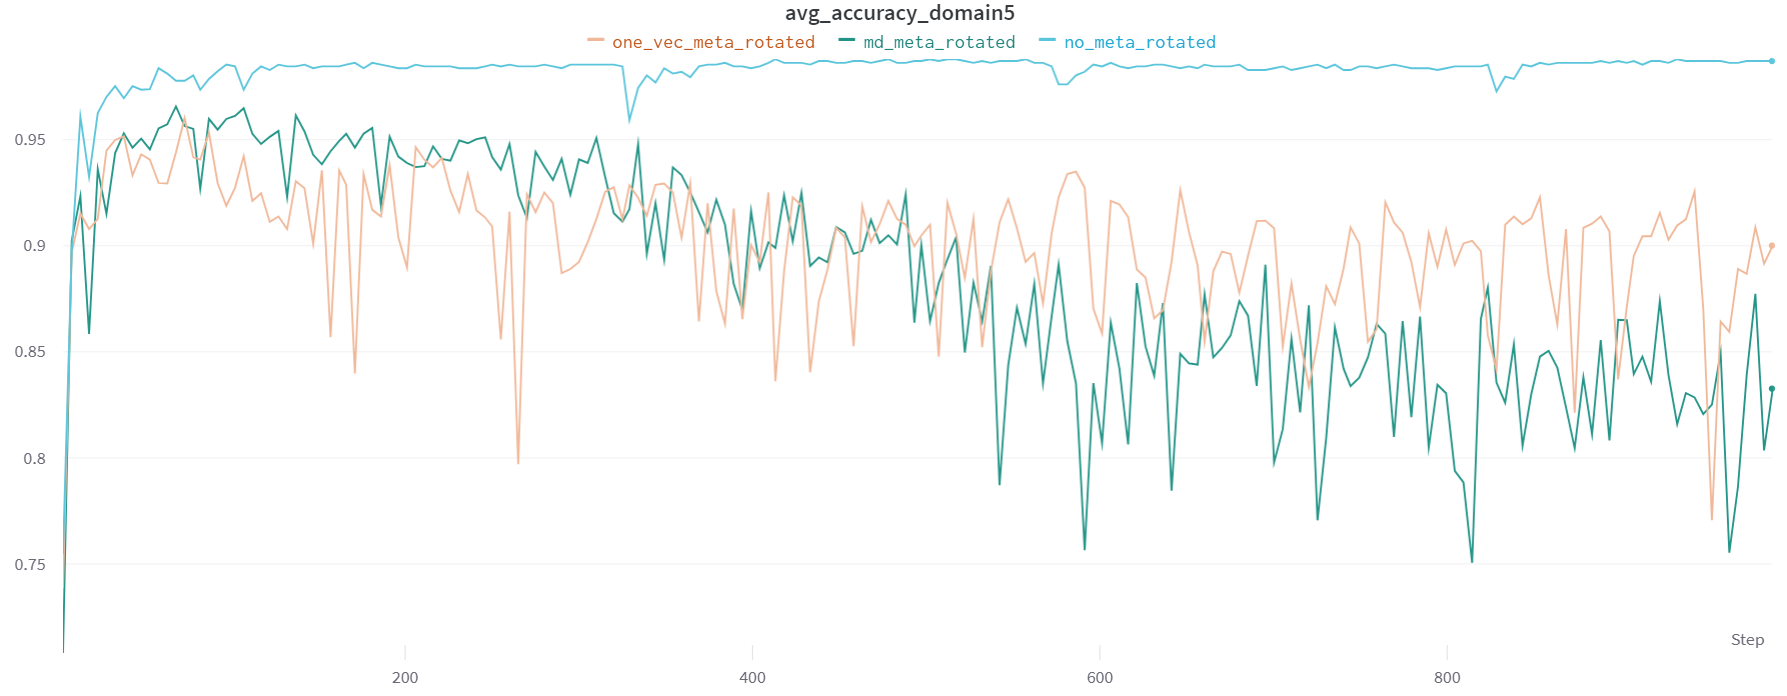
\includegraphics[width=1\linewidth]{images/results/avg_acc_val}
			\caption{The accuracy of each model over the RotatedMNIST validation set, function of training step.}
			\label{fig:rotated_avg_acc}
		\end{figure*}
		\begin{figure*}[h]
			\centering
			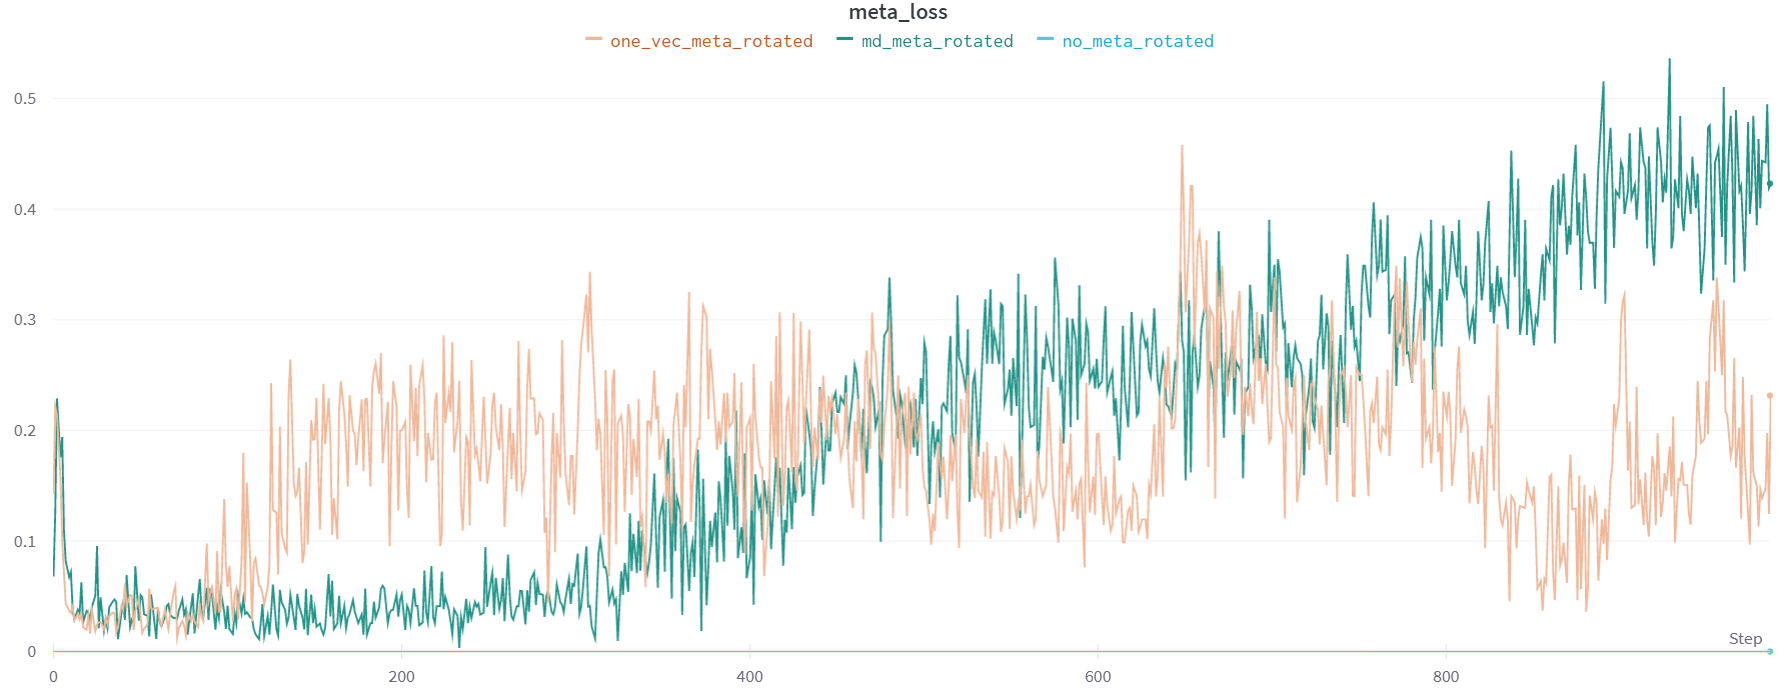
\includegraphics[width=1\linewidth]{images/results/meta_loss}
			\caption{The meta loss over the meta-validation set in RotatedMNIST, comparing the meta-calibration techniques. Since the regular ERM doesn't use meta-training, we set its value to zero.}
			\label{fig:rotated_meta_loss}
		\end{figure*}
		\begin{figure*}[h]
			\centering
			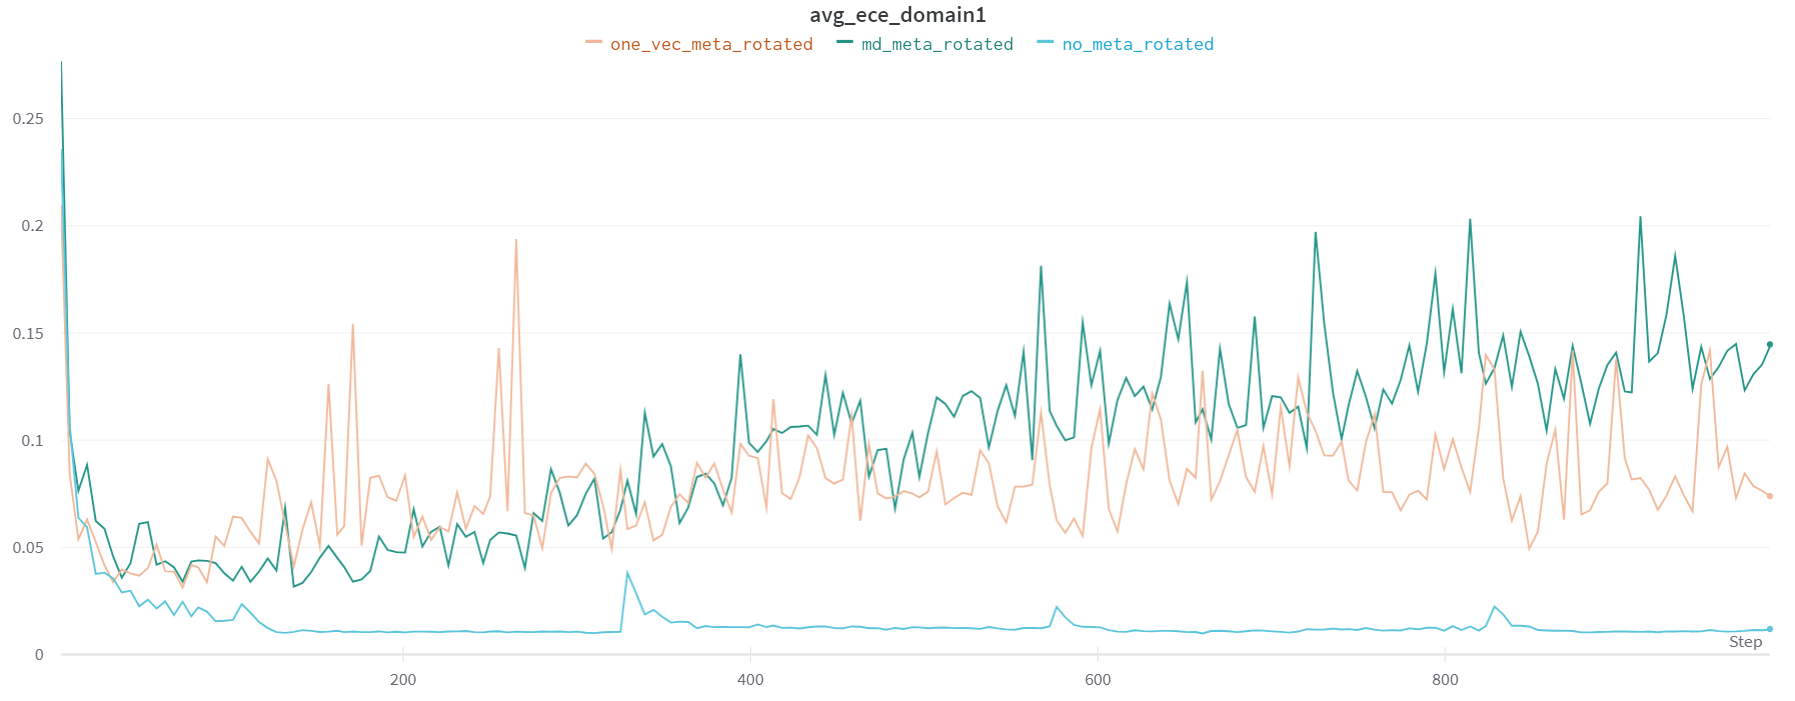
\includegraphics[width=1\linewidth]{images/results/avg_ece_val}
			\caption{The ECE calibration metric over the validation set in RotatedMNIST as a function of training step.}
			\label{fig:rotated_ece}
		\end{figure*}
	
	\subsection{ColoredMNIST}
		Figure \ref{fig:colored_avg_acc} shows the accuracy of the different models, measured periodically during training over the validation set. The effect of overfitting caused by the artificially synthesized confounders is noticable. It seems that ERM and the classic one-vector variant of the meta-calibrated model achieve similar results of $\approx 74\%$, while the new multi-domain variant has consistently lower accuracy by $0.1\%$.\\
		As for calibration, in figure \ref{fig:colored_ece} we view the ECE metric of each of the models, again as a function of training step, and it shows the same trend: ERM and single-vector meta-calibration achieve similar results and the multi-domain variant lacks behind.
		
		\begin{figure*}[h]
			\centering
			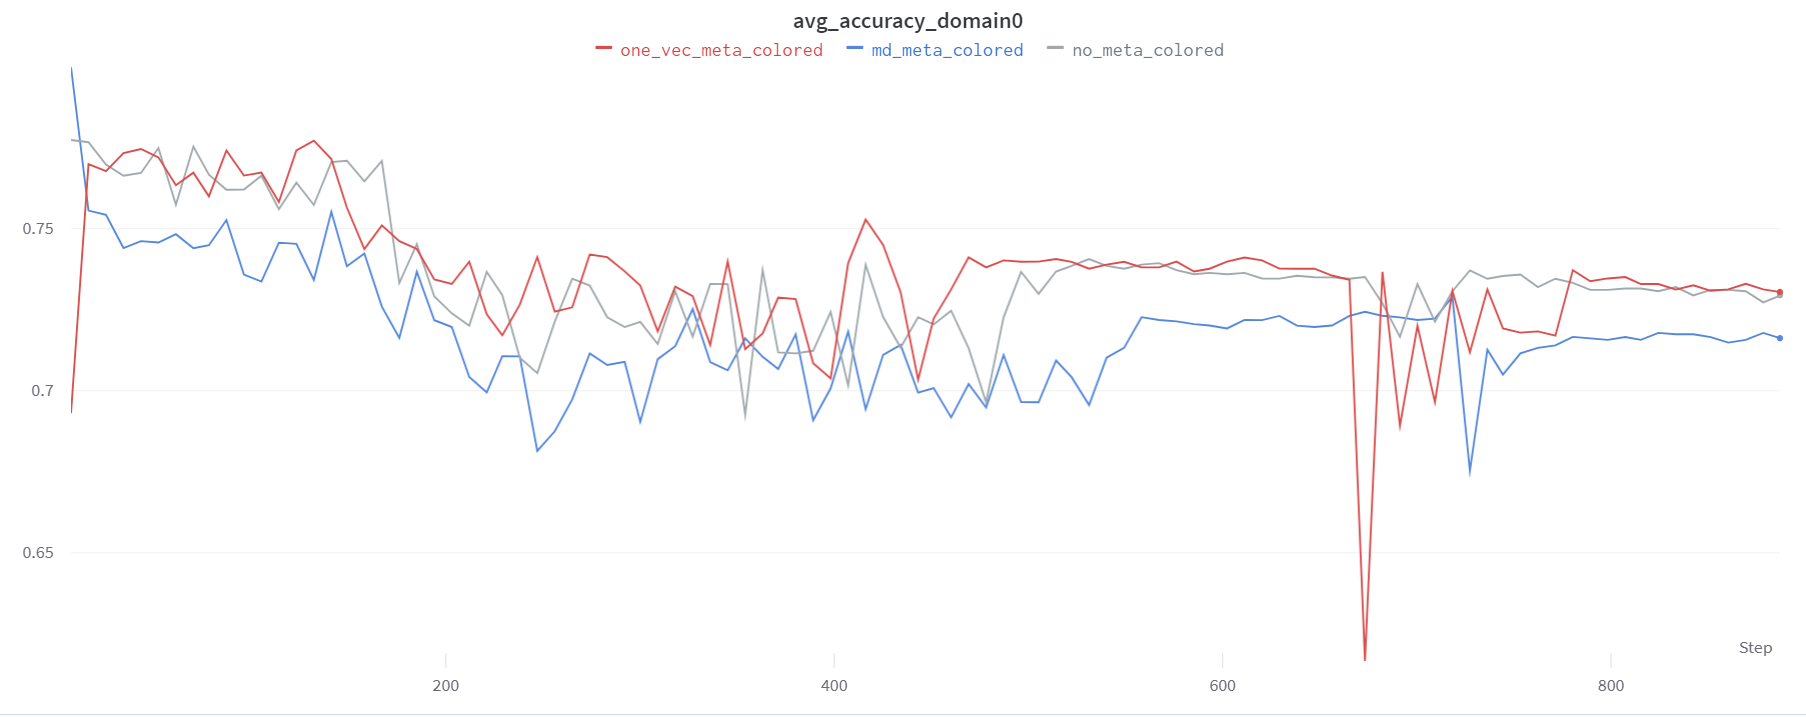
\includegraphics[width=1\linewidth]{images/results/avg_acc_val_colored}
			\caption{The accuracy of each model over the ColoredMNIST validation set, function of training step.}
			\label{fig:colored_avg_acc}
		\end{figure*}
		\begin{figure*}[h]
			\centering
			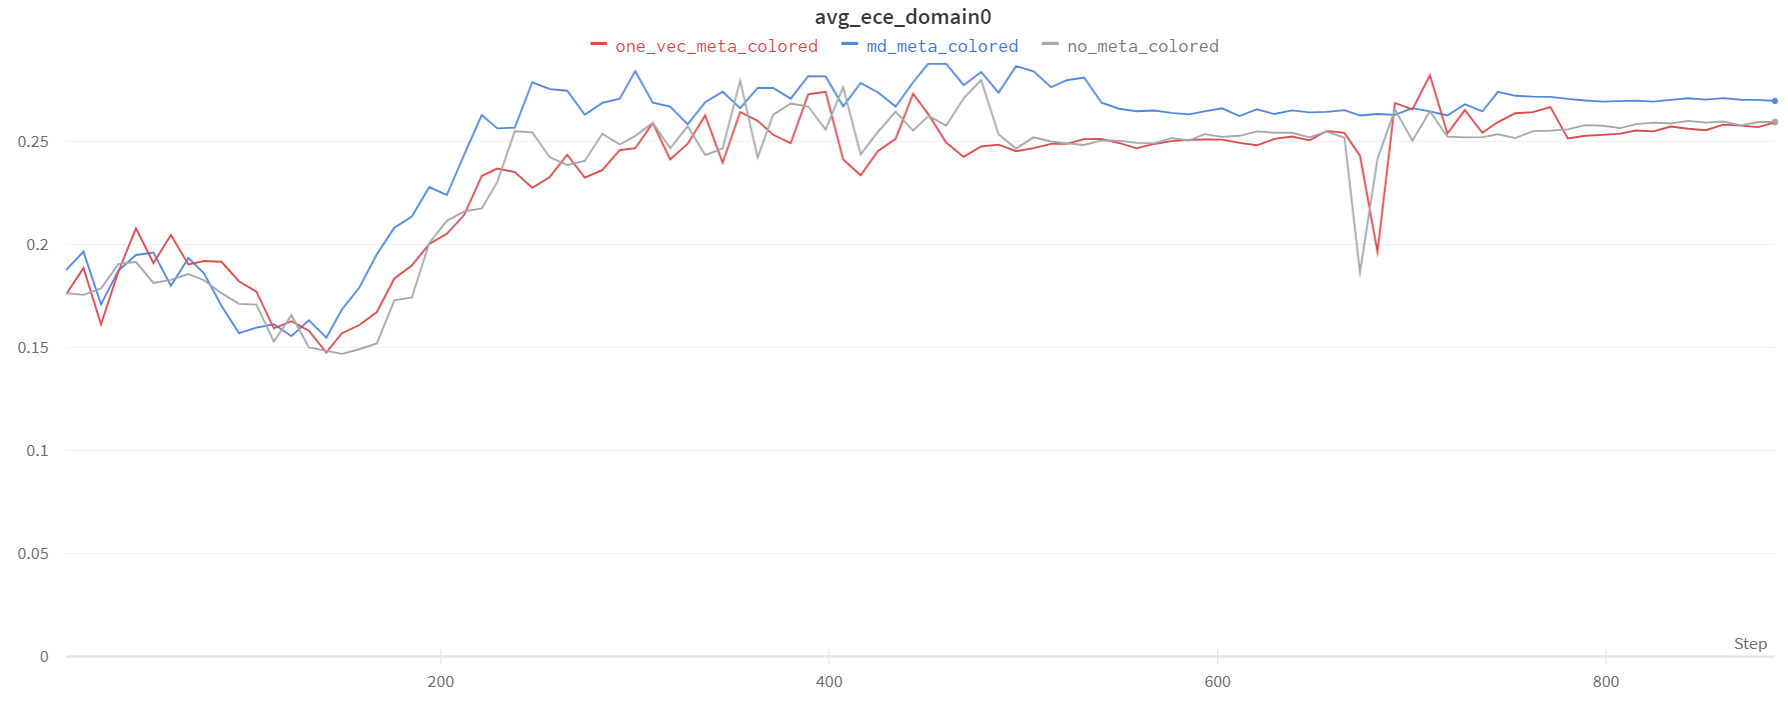
\includegraphics[width=1\linewidth]{images/results/avg_ece_val_colored}
			\caption{The ECE calibration metric over the validation set in ColoredMNIST as a function of training step.}
			\label{fig:colored_ece}
		\end{figure*}
	
	\subsection{CorruptedCIFAR10}
		We examined our new calibration method and the old "one vector method", in all combinations of possible data setups in which the train and meta-validation sets are either uni-domain (UD) or multi-domain (MD). The domains used for the MD test results are disjoint from the ones used during training.\\
		The pure results can be seen in tables \ref{tab:MD_train_UD_meta}, \ref{tab:MD_train_MD_meta} and \ref{tab:UD_train}. It seems that the new method outperforms the original single-vector method in the UD ece and in the avg MD ece. On the other hand, it is worse on the worst domain in each metric, and fails when we use an MD meta set.
		
		
		\begin{table*}
			\centering
			\begin{tabular}{ccccccc}
				\hline
				 & \textbf{UD err} & \textbf{UD ECE} & \textbf{MD max err} & \textbf{MD avg err} & \textbf{MD max ECE} & \textbf{MD avg ECE} \\
				\hline
				\textbf{no\_meta} & 0.134 & 9.09 & 0.282 & 0.175 & 19.9 & 12.1 \\
				\textbf{one\_vec\_meta} & 0.135 & 5.4 & 0.308 & 0.183 & 11.6 & 5.3 \\
				\textbf{md\_meta} & 0.151 & 3.22 & 0.342 & 0201 & 12.1 & 4.2 \\\hline
			\end{tabular}
			\caption{Results over the CorruptedCIFAR10 dataset, where the train set is multi-domain and the meta-validation set is uni-domain.}\label{tab:MD_train_UD_meta}
		\end{table*}

		\begin{table*}
			\centering
			\begin{tabular}{ccccccc}
				\hline
				& \textbf{UD err} & \textbf{UD ECE} & \textbf{MD max err} & \textbf{MD avg err} & \textbf{MD max ECE} & \textbf{MD avg ECE} \\
				\hline
				\textbf{no\_meta} & 0.134 & 9.09 & 0.282 & 0.175 & 19.9 & 12.1 \\
				\textbf{one\_vec\_meta} & 0.137 & 5.64 & 0.29 & 0.181 & 6.3 & 5.4 \\
				\textbf{md\_meta} & 0.16 & 8.87 & 0.366 & 0.211 & 15 & 8.7 \\\hline
			\end{tabular}
			\caption{Results over the CorruptedCIFAR10 dataset, where the train set is multi-domain and the meta-validation set is multi-domain. Note that the no\_meta method is equivalent to tabel \ref{tab:MD_train_UD_meta}}\label{tab:MD_train_MD_meta}
		\end{table*}

		\begin{table*}
			\centering
			\begin{tabular}{ccccccc}
				\hline
				& \textbf{UD err} & \textbf{UD ECE} & \textbf{MD max err} & \textbf{MD avg err} & \textbf{MD max ECE} & \textbf{MD avg ECE} \\
				\hline
				\textbf{no\_meta} & 0.49 & 4.17 & 0.786 & 0.243 & 74 & 21.2 \\
				\textbf{MD\_meta} & 0.63 & 10.73 & 0.574 & 0.212 & 26.9 & 8.7 \\
				\textbf{UD\_meta} & 0.69 & 1.22 & 0.615 & 0.256 & 35.5 & 13.1 \\\hline
			\end{tabular}
			\caption{Results over the CorruptedCIFAR10 dataset, where the train set is uni-domain. Therefore the md\_meta is equivalent to the one\_vec\_meta.}\label{tab:UD_train}
		\end{table*}
	
\section{Discussion and future work}
\label{sec:Discussion}
\subsection{MNIST}
The results we have received in the MNIST portion of this project were not as we expected. \cite{bohdal2021meta} showed tremendous gains to calibration from the meta-LS technique, which were not reproduced in our experiments. Note several major differences between our experimental setup and theirs:
\begin{itemize}
	\item Different dataset: for multi-domain training we leveraged the ColoredMNIST and RotatedMNIST datasets which are fundamentally different from the CIFAR dataset used in \cite{bohdal2021meta} and in the other part of our project.
	\item Different architecture: while both are convolutional neural networks, we used the architecture advised by DomainBed and \cite{bohdal2021meta} used ResNet-18.
	\item Different training specifics: Learning rate, number of epochs and optimization decisions are naturally different between the implementations.
\end{itemize}
These differences raise possible explenations for the gap in results. Firstly, optimization hyper-parameters may be crucial and architecture-dependent for the meta-calibration task, especially since the number of parameters is small. Furthermore, we note that the MNIST dataset is generally an easy classification task, for which many models acheive extremely high levels of accuracy. Hence, high confidence is not necessarily unjustified, and as we have seen, leads to low calibration error (see figures \ref{fig:rotated_ece}, \ref{fig:colored_ece}). This is plausibly the primary cause to the under-performance of the meta-calibration-trained models in our experiments on MNIST variants.\\
The new variant for meta-optimization we used in this project, the multi-domain label smoothing technique, didn't show any improvements over the other methods in the MNIST section. Perhaps this is the same issue as the underperformance of the single-vector meta-calibration; another option is that splitting the parameters to different domains doesn't yield benefit but rather adds unnecessary noise to the training process.\\

\subsection{CIFAR}
Unlike the previous section, noticable gains in calibration can be seen in our experiments over the CorruptedCIFAR10 dataset when using the meta calibration methods. Additionally, the new multi-domain adjusted version of meta-calibration yields the best ECE when fitted with a multi-domain training set and single-domain meta-validation set. Thus, it seems that the new method has great potential and can be useful when trying to get calibrated models. Further research is required to determine whether our method has any significant advantage over the existing ones.

\subsection{Future work}
Firstly, an obvious continuation is experimentation of the same models using other multi-domain datasets and tasks, as the calibration techniques may only be effective for difficult tasks. Other paths forward include different meta-parameters instead/in addition to label smoothing, such as regularization or hyper-parameters of loss functions.
	
	
\pagebreak
\section{Conclusion}
\label{sec:Conclusion}
Out-of-domain calibration is necessary in real-world applications to provide predictions with reliable confidence output. In this project, we tested a meta-training technique which trains models to be well-calibrated, in a new setting of multiple training/test domains. We implemented an adjusted meta-training version for the multi-domain case and performed experiments over three datasets. The CorruptedCIFAR10 dataset provided promising results, showing improved calibration in some cases over the existing method. However, datasets derived from MNIST led to poor results with both the new technique and the original one. We believe additional research may leverage the multi-domain-adjusted technique to train well-calibrated models efficiently.

\bibliographystyle{acl_natbib}
\bibliography{references}


\end{document}
